\newpage
\section{Implementação de um \emph{firewall} na NetFPGA}
\label{sec:impl}

Nesta seção apresentamos o \emph{firewall} que implementamos na
NetFPGA.  Apresentamos os detalhes de implementação e explicamos os
fundamentos para que o leitor possa implementar seu próprios
projetos.  Nosso \emph{firewall} tem várias simplificações para
torná-lo mais didático.  Em particular, o \emph{firewall} filtra
apenas pacotes TCP e o único tipo de regra que suporta é filtragem
por porta de destino.  Outra simplificação é que o \emph{firewall}
suporta filtragem de até quatro portas.  As razões destas
simplificações ficarão claras durante as discussões nesta seção.
Apesar das simplificações, esperamos que leitores sejam capazes de
estender o \emph{firewall} apresentado utilizando o conteúdo do
tutorial.

Esta seção é dividida em cinco partes complementares.  Na
\secstr~\ref{sec:impl.pkt} nós discutimos o processamento de pacotes
na NetFPGA, na \secstr~\ref{sec:impl.mod} discutimos como pacotes
podem ser modificados em trânsito, na \secstr~\ref{sec:impl.mem}
mostramos como um módulo pode utilizar a memória SRAM e na
\secstr~\ref{sec:impl.regs} mostramos como definir registradores e
acessá-los através de programas de espaço de usuário.  Por fim, na
\secstr~\ref{sec:impl.test} apresentamos o sistema de testes
disponível no \emph{software} da NetFPGA.

A maior parte do código apresentado neste material refere-se aos
arquivos Verilog (\ssf{.v}) usados para simulação e síntese do
\emph{hardware}.  A sintaxe para comentários em Verilog é idêntica à
de C.\footnotemark{}  O \emph{software} da NetFPGA possui também
\emph{scripts} Bash (\ssf{.sh}), Perl (\ssf{.pl}) e Python
(\ssf{.py}), que adotam o caractere (\ssf{\#}) para comentários de
linha.  Salvo quando indicado, iremos mostrar código retirado do
módulo principal do nosso \emph{firewall}, em
\ssf{netfpga/projects/firewall/src/firewall.v}.

\footnotetext{Algumas dicas para programação em Verilog são
apresentadas no apêndice A.}

\input{41impl.pkt}

\input{42impl.mod}

\subsection{Acesso à memória SRAM}
\label{sec:impl.mem}

Nosso módulo utiliza a memória SRAM para armazenar as portas
bloqueadas e decidir quais pacotes filtrar.  No sexto estado do
processamento de um pacote emitimos uma requisição de leitura para o
endereço \ssf{SRAM\_PORTS\_ADDR}, que contem as portas TCP
bloqueadas.  No sétimo estado esperamos a leitura completar e então
utilizamos o dado lido para verificar se o pacote precisa ser
descartado ou não.

Nosso \emph{firewall} emite operações de leitura da memória para o
módulo \ssf{sram\_arbiter}, que intermedia o acesso à memória SRAM.
As linhas de comunicação do nosso \emph{firewall} com o
\ssf{sram\_arbiter} ilustram a interface de acesso à memória.

\begin{verilogcode}
      output reg                       sram_rd_req,
      output reg [SRAM_ADDR_WIDTH-1:0] sram_rd_addr,
      input [DATA_WIDTH-1:0]           sram_rd_data,
      input                            sram_rd_ack,
      input                            sram_rd_vld,
      output reg                       sram_wr_req,
      output reg [SRAM_ADDR_WIDTH-1:0] sram_wr_addr,
      output reg [DATA_WIDTH-1:0]      sram_wr_data,
      input                            sram_wr_ack,
\end{verilogcode}

O \ssf{sram\_arbiter} pode receber uma requisição de leitura ou
escrita por ciclo de relógio.  Requisições de leitura são indicadas
ligando \ssf{sram\_rd\_req} e informando o endereço a ser lido em
\ssf{sram\_rd\_addr}.  No próximo ciclo de relógio o
\ssf{sram\_arbiter} indica se a requisição foi recebida com sucesso
ligando o sinal \ssf{sram\_rd\_ack}.  Como leituras demoram alguns
ciclos para serem atendidas, o módulo que pediu a leitura deve
esperar os dados serem retornados e disponibilizados pelo
\ssf{sram\_arbiter}.  O \ssf{sram\_arbiter} informa que os dados
estão disponíveis em \ssf{sram\_rd\_data} ligando
\ssf{sram\_rd\_vld}.

Requisições de escrita são indicadas ligando \ssf{sram\_wr\_req},
informando o endereço a ser escrito em \ssf{sram\_wr\_addr} e
informando o dado a ser escrito em \ssf{sram\_wr\_data}.  O
\ssf{sram\_arbiter} indica se a requisição foi recebida com sucesso
ligando o sinal \ssf{sram\_wr\_ack}.  Como o dado a ser escrito é
armazenado pelo \ssf{sram\_arbiter}, o módulo que fez a requisição
de escrita não precisa esperar mais nenhuma confirmação do
\ssf{sram\_arbiter}.  Se ambos os sinais \ssf{sram\_rd\_req} e
\ssf{sram\_wr\_req} estiverem ligados, nosso \ssf{sram\_arbiter}
prioriza a requisição de escrita.  A SRAM usada na NetFPGA garante
que leituras realizadas após escritas lerão o dado atualizado.

A interface que exportamos em nosso \ssf{sram\_arbiter} é
simplificada.  Como descrito na seção~\ref{sec:arch.hw}, a NetFPGA
possui dois bancos de memórias SRAM, cada um com $2^{19}$ linhas de
36~bits.  Nosso \ssf{sram\_arbiter} combina os dois bancos para
apresentar uma abstração de memória de $2^{19}$ linhas de 64~bits.
Usamos 8~bits de cada linha como bits de paridade, calculados e
verificados automaticamente pelo \ssf{sram\_arbiter}.

\begin{verilogcode}
   // sram_arbiter.v
   generate
      genvar m;
      for(m = 0; m < 8; m = m+1) begin: calc_par_bits
      assign parbit[m] = wr_data[m*8] ^ wr_data[m*8+1] ^
            wr_data[m*8+2] ^ wr_data[m*8+3] ^ wr_data[m*8+4] ^
            wr_data[m*8+5] ^ wr_data[m*8+6] ^ wr_data[m*8+7];
      end // wr_data is 64 bits wide
   endgenerate 
   generate
      genvar l;
      for(l = 0; l < 8; l = l+1) begin: expand_wr_data
         assign wr_data_exp[(l+1)*9-1 : l*9] =
            {wr_data[(l+1)*8-1:l*8], parbit[l]};
         end // wr_data_exp is 72 bits wide (36*2)
   endgenerate
\end{verilogcode}

Para acessar as duas memórias simultaneamente duplicamos os sinais
de requisição de escrita ou leitura e os endereços para os dois
bancos de memória.  Para requisições de escrita escrevemos metade
dos dados em cada banco e para requisições de leitura concatenamos
os dados dos dois bancos.  Abaixo mostramos o código para realizar
estas operações.  Este código fica dentro do módulo \ssf{nf2\_core}.
O módulo \ssf{nf2\_core} é o módulo raiz do \emph{software} da
NetFPGA e comunica diretamente com os pinos do FPGA.  O
\ssf{nf2\_core} conecta os pinos do FPGA conectados às memórias SRAM
ao \ssf{sram\_arbiter} da seguinte forma.

\begin{verilogcode}
// nf2_core.v
// hardware pins       sram_arbiter
assign sram1_wr_data = wr_data_exp[`SRAM_DATA_WIDTH-1:0];
assign sram2_wr_data = wr_data_exp[2*`SRAM_DATA_WIDTH-1:`SRAM_DATA_WIDTH];
assign sram1_we      = sram_we; // 0 for write, 1 for read
assign sram2_we      = sram_we;
assign sram1_addr    = sram_addr;
assign sram2_addr    = sram_addr;
// sram_arbiter        hardware pins
assign sram_rd_data  = {sram2_rd_data, sram1_rd_data};
\end{verilogcode}

O \ssf{sram\_arbiter} pode ser modificado para permitir acesso mais
eficiente à memória caso a aplicação tenha um padrão específico de
acessos.  Por exemplo, é possível modificar as atribuições acima
para permitir ler endereços distintos em cada banco de SRAM.  A SRAM
também provê um mecanismo para permitir escritas parciais,
escolhendo quais bytes devem ser escritos em uma requisição de
escrita.\footnotemark{}

\footnotetext{Não mostramos esta funcionalidade no texto.  Nossa
implementação não suporta escritas parciais.  Escritas parciais
poderiam ser controladas configurando o valor das linhas
\sssf{sram\_bw} no \sssf{sram\_arbiter}.}

Para exemplificar o controle de acesso à SRAM num nível mais baixo,
iremos explicar o tratamento de uma requisição de leitura
(requisições de escrita são mais simples).  Quando o
\ssf{sram\_arbiter} recebe uma requisição de leitura, ele desabilita
escrita ligando o sinal \ssf{sram\_we} (este sinal possui lógica
negativa), repassa o endereço a ser lido ao \emph{hardware} e
confirma a requisição de leitura.

\begin{verilogcode}
   // sram_arbiter.v
   else if(sram_rd_req) begin
      hw_we <= 1'b1;                // read
      hw_addr <= sram_rd_addr;
      sram_rd_ack <= sram_rd_req;   // acknowledge read request
      sram_wr_ack <= 0;             // do not acknowledge write
      rd_vld_early3 <= sram_rd_req; // data back in three cycles
      ...
   end
\end{verilogcode}

Como o dado demora dois ciclos para ser retornado da SRAM após a
requisição, o \ssf{sram\_arbiter} possui um \emph{pipeline} interno
para esperar os dados serem retornados pela SRAM.  Após dois ciclos
o \ssf{sram\_arbiter} armazena o dado lido no registrador
\ssf{sram\_rd\_data} e encaminha este registrador para o
\emph{firewall} no terceiro ciclo de relógio após a requisição.

\begin{verilogcode}
   // sram_arbiter.v
   rd_vld_early2 <= rd_vld_early3; // waited 1
   rd_vld_early1 <= rd_vld_early2; // waited 2
   if(rd_vld_early1) begin // memory sending data this cycle, storing
      if(parity_check)
         sram_rd_data <= rd_data_exp_parsed; // no parity bits
      else
         sram_rd_data <= 64'hdeadfeeddeadfeed;
   end
   sram_rd_vld <= rd_vld_early1;   // data is here, set valid bit
\end{verilogcode}


\subsection{Registradores e interface PCI}
\label{sec:impl.regs}

Nosso projeto define quatro registradores de \emph{software}, um
para cada porta de destino que deve ser bloqueada.  Estes
registradores de \emph{software} podem ser configurados
dinamicamente a partir do espaço de usuário.  Nós definimos os
registradores no arquivo XML de configuração do nosso projeto como
abaixo.

\begin{minted}{xml}
<!-- netfpga/projects/firewall/include/project.xml -->
<nf:name>firewall</nf:name>
   <nf:prefix>firewall</nf:prefix>
   <nf:location>udp</nf:location>
   <nf:description>Registers for minifirewall</nf:description>
   <nf:blocksize>128</nf:blocksize>
   <nf:registers>
      <nf:register>
         <nf:name>dport1</nf:name>
         <nf:description>Blocked port 1</nf:description>
         <nf:type>generic_software32</nf:type>
      </nf:register>
      ...
   </nf:registers>
\end{minted}

O programa \ssf{nf\_register\_gen} processa os arquivos XML de
configuração de todos os módulos de um projeto, gera um
identificador para cada módulo, calcula requisitos de armazenamento
para os registradores de cada módulo e gera endereços virtuais para
cada registrador.\footnotemark{}  O endereço virtual de um
registrador é composto do identificador do módulo onde foi declarado
e de seu deslocamento dentro do bloco de memória reservado aos
registradores do módulo.  Como nosso \emph{firewall} possui quatro
registradores de 32 bits para armazenar as portas TCP que estão
bloqueadas, definimos um bloco de registradores de 128 bits
(\ssf{blocksize} na configuração acima).  O tamanho do bloco de
registradores define a quantidade de bits necessárias para a parte
de deslocamento do endereço dos registradores.

\footnotetext{O arquivo XML com a configuração global do
\emph{firewall} está em
\url{netfpfa/projects/firewall/include/project.xml}.  Arquivos com a
configuração dos módulos estão no mesmo diretório.}

O \ssf{nf\_register\_gen} gera cabeçalhos Verilog, C, Python e Perl
contendo constantes que permitem endereçar os registradores em cada
uma destas linguagens.  Os arquivos de cabeçalho são necessários
para compilação de programas de usuário e sintetização do projeto em
\emph{hardware}.  O \ssf{nf\_register\_gen} pode ser executado com o
comando seguinte (os cabeçalhos são criados dentro da pasta
\ssf{netfpga/projects/firewall/lib/}):

\begin{minted}{bash}
netfpga/bin/nf_register_gen.pl --project firewall
\end{minted}

% \begin{table}[h]
% \centering
% \begin{tabular}{|l|l|l|}
% \hline
% \textbf{Macro}       & \textbf{Endereço Verilog} & \textbf{Endereço C} \\ \hline
% FIREWALL\_DPORT1 & 5'h0                      & 0x2000000           \\ \hline
% FIREWALL\_DPORT2 & 5'h1                      & 0x2000004           \\ \hline
% FIREWALL\_DPORT3 & 5'h2                      & 0x2000008           \\ \hline
% FIREWALL\_DPORT4 & 5'h3                      & 0x200000c           \\ \hline
% \end{tabular}
% \label{tab:impl.firewall.regs}
% \caption{Endereços virtuais em arquivos de cabeçalho C e Verilog dos registradores do firewall.}
% \end{table}

Os endereços virtuais de registradores em programas do usuário
possuem 28~bits e independem do tipo do registrador (contador,
\emph{software}, ou \emph{hardware}).  Como a NetFPGA interage com
sistemas operacionais de 32~bits, registradores maiores que 32 bits
são particionados em múltiplas palavras de 32~bits segundo o esquema
mostrado nas colunas ``64~bits'' e ``128~bits'' na
tabela~\ref{table:impl.regs.width}.

\begin{table}[h]
\centering
\begin{tabular}{llllll}
\multicolumn{2}{c}{\textbf{32 bits}} & \multicolumn{2}{c}{\textbf{64 bits}} & \multicolumn{2}{c}{\textbf{128 bits}} \\ \hline
\textbf{Macro}     & \textbf{Endereço} & \textbf{Macro}         & \textbf{Endereço} & \textbf{Macro}            & \textbf{Endereço} \\ \hline
\ssf{EX\_REG} & 0x2000004         & \ssf{EX\_REG\_LO} & 0x2000004         & \ssf{EX\_REG\_1\_LO} & 0x2000004   \\
                   &                   & \ssf{EX\_REG\_HI} & 0x2000008         & \ssf{EX\_REG\_1\_HI} & 0x2000008   \\
                   &                   &                        &                   & \ssf{EX\_REG\_2\_LO} & 0x200000c   \\
                   &                   &                        &                   & \ssf{EX\_REG\_2\_HI} & 0x2000010   \\
\end{tabular}
\caption{Exemplo do esquema de geração de nomes para registradores maiores que 32 bits.}
\label{table:impl.regs.width}
\end{table}

Registradores de \emph{software} podem ser escritos lidos e escritos
utilizando as funções \ssf{readReg} e \ssf{writeReg} definidas na
biblioteca de funções da NetFPGA (em \ssf{netfpga/lib}).  Por
exemplo, no nosso programa de configuração dinâmica das portas
bloqueadas, \ssf{nffw}, temos:

\begin{minted}{c}
   // netfpga/projects/firewall/sw/nffw.c
   writeReg(&nf2, FIREWALL_DPORT0_REG, dropped[0]);
   ...
   readReg(&nf2, FIREWALL_DPORT0_REG, &check[0]);
\end{minted}

A memória SRAM também pode ser acessada pela interface de
registradores.  A primeira palavra da memória SRAM é mapeada no
endereço virtual \ssf{SRAM\_BASE\_ADDR}, e outras palavras podem ser
acessadas indiretamente a partir de \ssf{SRAM\_BASE\_ADDR}.  O
seguinte exemplo zera as dez primeiras palavras da memória:

\begin{minted}{c}
   for(i = 0; i < 10; i++)
      unsigned offset = i*4; // 4 bytes per word
      writeReg(&nf2, SRAM_BASE_ADDR + offset, 0);
\end{minted}

Chamadas de função como \ssf{writeReg} enviam uma requisição de
escrita em registrador para a NetFPGA.  Essa requisição é recebida
pelo barramento PCI.  Para facilitar o processamento de requisições
de escrita e leitura dos registradores, podemos usar o módulo
\ssf{generic\_regs}.  O módulo \ssf{generic\_regs} é padrão no
pacote de \emph{software} da NetFPGA e é instanciado dentro dos
módulos que compõem o \emph{pipeline} de processamento.

Quando instanciamos o \ssf{generic\_regs}, definimos o número de
registradores e as linhas conectadas a cada registrador.  Definimos
também em qual módulo ele está sendo instanciado (parâmetro
\ssf{TAG}).  Esta informação permite à instância do
\ssf{generic\_regs} identificar os endereços dos registradores do
módulo e quais requisições de escrita e leitura em registradores
deve tratar.

\begin{verilogcode}
   generic_regs
   #(
      .TAG               (`FIREWALL_BLOCK_ADDR), // module ID
      .NUM_SOFTWARE_REGS (4),                    // number of sw regs
      ...
   ) module_regs (
      .reg_req_in       (reg_req_in),      // register bus input lines
      .reg_ack_in       (reg_ack_in),
      .reg_rd_wr_L_in   (reg_rd_wr_L_in),
      .reg_addr_in      (reg_addr_in),
      .reg_data_in      (reg_data_in),
      .reg_src_in       (reg_src_in),
      .reg_req_out      (reg_req_out),     // register bus output lines
      .reg_ack_out      (reg_ack_out),
      .reg_rd_wr_L_out  (reg_rd_wr_L_out),
      .reg_addr_out     (reg_addr_out),
      .reg_data_out     (reg_data_out),
      .reg_src_out      (reg_src_out),
      .counter_updates  (),                // register definitions
      .counter_decrement(),
      .software_regs    ({dport1, dport2, dport3, dport4}),
      .hardware_regs    (),
      ...
    );
\end{verilogcode}

As requisições de leitura e escrita em registradores recebidas pelo
barramento PCI são inseridas no barramento de registradores.  O
barramento de registradores é paralelo ao barramento de
encaminhamento.  Como no barramento de encaminhamento, cada
instância do módulo \ssf{generic\_regs} tem sinais de entrada
(sufixo \ssf{\_in}), para receber requisições do módulo anterior, e
de saída (sufixo \ssf{\_out}), para repassar as requisições ao
próximo módulo.  Ilustramos o barramento de registradores na
figura~\ref{fig:impl.regs.bus}.  A linha \ssf{req} indica se as
outras linhas carregam uma requisição válida.  As linhas \ssf{addr}
especificam o endereço virtual do registrador.  A linha
\ssf{rd\_wr\_L} indica se a requisição é de leitura ou escrita (com
lógica negativa, leitura quando ligado e escrita quando desligado) e
as linhas \ssf{data} contém o dado a ser escrito ou o dado lido.  A
linha \ssf{ack} indica se a requisição já foi tratada e as linhas
\ssf{src} indicam qual módulo tratou a requisição.

\begin{figure}
\centering
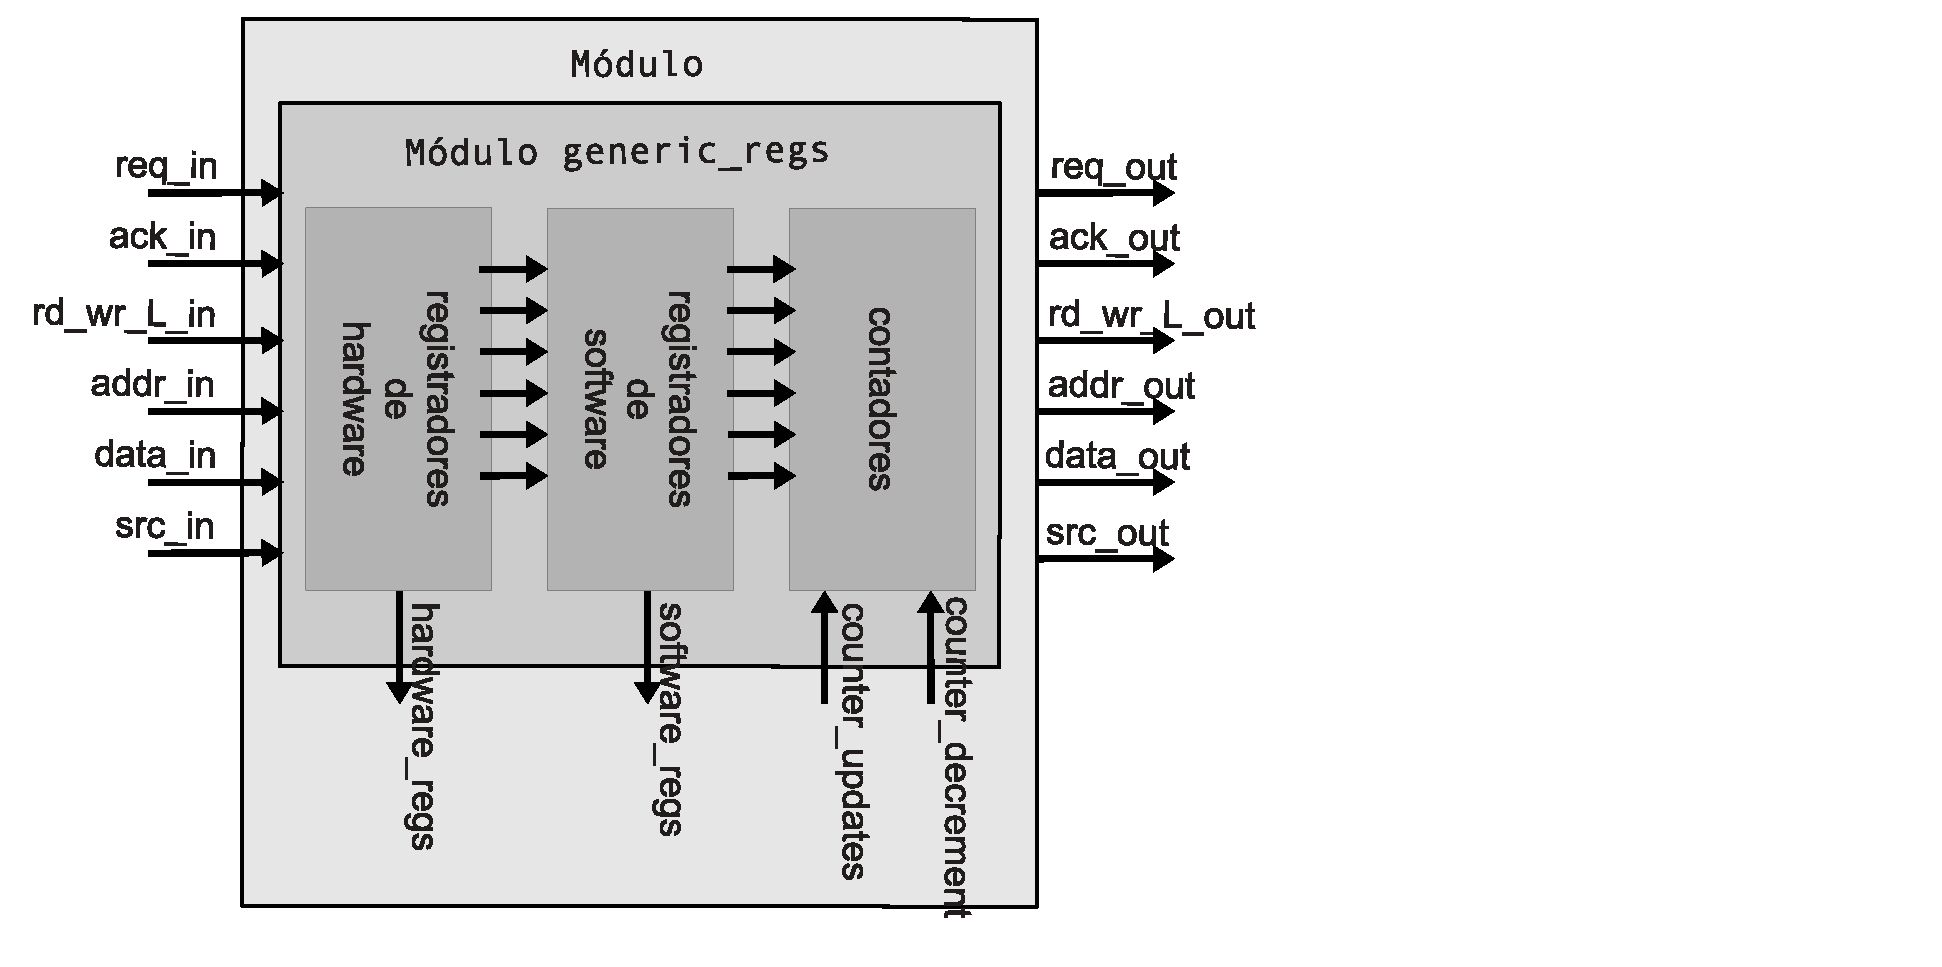
\includegraphics[scale=0.6,angle=0]{figures/modulos/genregister.eps}
\caption{Módulo \ssf{generic\_regs} e barramento de registradores.}
\label{fig:impl.regs.bus}
\end{figure}

O \ssf{nf\_register\_gen} gera blocos para armazenamento de
registradores automaticamente.  Para projetos com requisitos
específicos, é possível controlar o endereço base dos registradores
de cada módulo no arquivo XML de configuração do projeto.  Por
exemplo, para posicionar os registradores do nosso \emph{firewall}
no endereço \ssf{0x02000400} basta utilizar a configuração a seguir.

\begin{minted}{xml}
<!-- netfpga/projects/firewall/include/project.xml -->
<nf:memalloc layout="reference">
    <nf:group name="udp">
        <nf:instance name="firewall" base="0x02000400"/>
        ...
    </nf:group>
    ...
</nf:memalloc>
\end{minted}

Nosso \emph{firewall} lê as portas que devem ser filtradas da
memória SRAM (sexto estágio).  Esta decisão de projeto é didática,
para exemplificar a utilização da memória SRAM.  Num projeto real,
as portas poderiam ser lidas diretamente dos registradores
\ssf{dport0}, \ssf{dport1}, \ssf{dport2}, \ssf{dport3}.  Para que
possa ler as portas TCP bloqueadas da memória SRAM, nosso
\emph{firewall} precisa também gravar esta informação na memória.
Isto é realizado gravando os registradores na memória usando o
módulo \ssf{sram\_arbiter}.  Para detectar se as portas bloqueadas
foram modificadas, verificamos se o uma requisição de registrador
foi atendida (\ssf{reg\_ack\_out}) e se o endereço da requisição
pertence ao nosso módulo (\ssf{tag\_hit} e \ssf{addr\_good}).  Para
verificar se o endereço da requisição pertence ao nosso módulo,
utilizamos as constantes geradas pelo \ssf{nf\_register\_gen}.

\begin{verilogcode}
   always @(*) begin
      wr_data_next <= {dport3[15:0], dport2[15:0],
                       dport1[15:0], dport0[15:0]};
      wr_addr_next <= SRAM_PORTS_ADDR;
      if(tag_hit && addr_good && reg_ack_out)
         wr_req_next <= 1;
      else
         wr_req_next <= 0;
   end
   assign addr_block = reg_addr_out[`UDP_REG_ADDR_WIDTH-1:
                                    `FIREWALL_REG_ADDR_WIDTH];
   assign tag_hit = `FIREWALL_BLOCK_ADDR == addr_block;
   assign addr_good = reg_addr_out[`FIREWALL_REG_ADDR_WIDTH-1:0] >= 
    `FIREWALL_DPORT0 && reg_addr_out[`FIREWALL_REG_ADDR_WIDTH] <= 
    `FIREWALL_DPORT3;
\end{verilogcode}

As linhas \ssf{addr\_block} são construídas a partir do endereço da
requisição e contém o identificador do bloco de registradores (linha
10).  O identificador do bloco de registradores pode ser utilizado
para verificar se o registrador pertence ao nosso módulo (linha 12).
Por último, a linha \ssf{addr\_good} indica se o registrador escrito
é um dos registradores que armazena as portas TCP bloqueadas (linha
13).


\input{45impl.tst}

